\subsection{The homography, written as a linear system}
\label{sec:dlt}

The map~\eqref{eq:homography} is used as a black box in the counter. The installation procedure has to compute it, so the linear system is part of the system design even though PLC never re-solves it per frame. A point $(X,Y)$ on the front plane and a pixel $(u,v)$ are related by
\begin{equation}
\begin{bmatrix} u \\ v \\ 1 \end{bmatrix}
\sim
H
\begin{bmatrix} X \\ Y \\ 1 \end{bmatrix},
\qquad
H=
\begin{bmatrix}
h_{11} & h_{12} & h_{13} \\
h_{21} & h_{22} & h_{23} \\
h_{31} & h_{32} & h_{33}
\end{bmatrix}.
\label{eq:H}
\end{equation}
The scale of $H$ is free. Clearing the homogeneous scale gives the two equations
\begin{equation}
\begin{aligned}
u(h_{31}X+h_{32}Y+h_{33}) &= h_{11}X+h_{12}Y+h_{13},\\
v(h_{31}X+h_{32}Y+h_{33}) &= h_{21}X+h_{22}Y+h_{23}.
\end{aligned}
\label{eq:dlt-pair}
\end{equation}
Stacked over $n\ge 4$ correspondences and moved to one side, the coefficients of the nine unknowns form a $2n\times 9$ matrix $A$ with a row pair
\begin{equation}
\begin{aligned}
&(X,\; Y,\; 1,\; 0,\; 0,\; 0,\; -uX,\; -uY,\; -u),\\
&(0,\; 0,\; 0,\; X,\; Y,\; 1,\; -vX,\; -vY,\; -v)
\end{aligned}
\label{eq:dlt-rows}
\end{equation}
for each correspondence. The solution is the singular vector of $A$ belonging to the smallest singular value~\cite{hartley2004mvg}. RANSAC wraps that solve: draw four correspondences, fit, count how many of the remaining points fall within a pixel threshold, and keep the set with the largest count~\cite{fischler1981ransac}. The target that supplies the correspondences is the planar board of the geometric calibration, whose spacing is known in metres, so the singular vector comes out in the scale PLC assumes when it divides by $w$ and $h$.

Four non-collinear correspondences determine $H$. The target provides many more so that a mismatched corner can be rejected. The condition the installer checks is not the algebraic residual of $A$. It is the geometric residual on the rectified plane, in centimetres, because \Cref{prop:snap} is stated in centimetres. A fit that is excellent in pixels and scaled wrong by ten percent will alias the lattice. The tape check on $(w,h)$ and the residual check on $H$ are the same check read from two sides.

The same linear system says what a yaw of the truck does. A modest yaw of a still-planar face is absorbed into $H$ if $H$ is re-estimated, and it is a bias on every center if $H$ is the one computed at installation for a face that was square to the camera. The design does not re-estimate $H$ per truck. It relies on the gate geometry to keep the yaw inside the snap radius. A truck that approaches at a large angle violates that reliance, and the origin residual grows. The residual is the detector of the violation. It is not a substitute for re-estimating $H$ on a truck that is known to arrive askew. If a building's traffic pattern makes large yaw routine, the installation procedure changes and the mathematics of~\eqref{eq:dlt-rows} does not.

\subsection{Where the detection probability spends the misses}
\label{sec:detprob-discuss}

The snap and the gap rule see only the centers that survive~\eqref{eq:detprob}. The shape of that probability is the reason a uniform hole-filler would be the wrong rule. With $\beta=0$ the bottom row is kept with probability $0.70$, the top row with probability $0.84$, and a middle row with probability $0.96$. With $\beta=1$ those numbers fall by $0.18$, to $0.52$, $0.66$, and $0.78$, before the clip at $0.35$ ever binds. The clip binds only if a future model adds a further penalty. In the stated model the bottom row at full blur is still detected more often than not.

\begin{figure}[t]
\centering
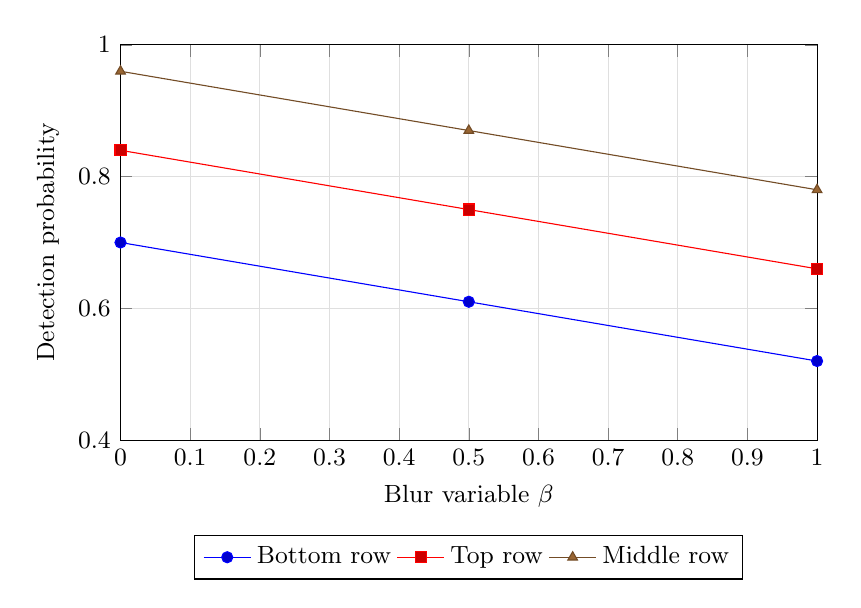
\begin{tikzpicture}
\begin{axis}[
  width=0.86\textwidth,
  height=6.6cm,
  xlabel={Blur variable $\beta$},
  ylabel={Detection probability},
  ymin=0.4, ymax=1.0,
  xmin=0, xmax=1,
  legend style={font=\small, at={(0.5,-0.24)}, anchor=north, legend columns=3},
  tick label style={font=\small},
  label style={font=\small},
  grid=major,
  grid style={gray!25}
]
\addplot+[mark=*] coordinates {(0,0.70) (0.5,0.61) (1,0.52)};
\addplot+[mark=square*] coordinates {(0,0.84) (0.5,0.75) (1,0.66)};
\addplot+[mark=triangle*] coordinates {(0,0.96) (0.5,0.87) (1,0.78)};
\legend{Bottom row, Top row, Middle row}
\end{axis}
\end{tikzpicture}
\caption{Detection probability~\eqref{eq:detprob} against blur, for a stack tall enough to have a distinct bottom, middle, and top. The gap rule is asked to repair the bottom curve, not the middle one.}
\label{fig:detprob}
\end{figure}

On a front face of four rows and three columns with every cell occupied, twelve crates, the expected number of misses at $\beta=0$ is
\begin{equation}
3(1-0.70)+3(1-0.84)+6(1-0.96)
= 0.90+0.48+0.24
= 1.62.
\label{eq:expected-miss}
\end{equation}
At $\beta=1$ the same sum is $3(0.48)+3(0.34)+6(0.22)=3.78$. A middle miss is the miss the two-neighbor rule is built to restore: the cell above and the cell below exist. A bottom miss has no lower neighbor. It is restored only when both lateral neighbors were detected, which on a three-column bottom row is true for the middle cell and only half-supported for the two ends. The rule is therefore a better repair of an interior hole than of a shadowed corner. Equation~\eqref{eq:expected-miss} says there is about one and a half misses to repair on a clean frame of that size, and nearly four on a blurred one. False positives arrive at a Poisson mean of $0.35$, an order of magnitude smaller than the blur-induced misses and large enough, across five independent frames, to supply the phantom cells that PLC-passage unions. The asymmetry is the design reason for trusting one frame.

The expected miss count is not the expected counting error. A miss that the gap rule restores costs nothing. A miss at a corner that the rule cannot see costs $\hat{d}$. A false positive that lands in an empty cell and acquires a second neighbor costs $\hat{d}$ the other way. The tables in Chapter~\ref{ch:system} are the net of those three effects. The expectation~\eqref{eq:expected-miss} only explains why the net is not zero and why it depends on which row was lost.

\subsection{The worked grid, drawn}
\label{sec:grid-drawn}

\Cref{fig:grid} draws~\eqref{eq:example-grid} before and after the pass~\eqref{eq:gap}. The occupied cells are the ten true front crates. The cell that the rule adds is the middle of the top row, which has a neighbor below and a neighbor to the right. The corner cell of that row has, at the moment it is visited, only the neighbor below, so it stays empty. The drawing is the whole of the positive bias on this stack: one invented front cell, times a depth of two, is two invented crates, before any missed detection is put back. When the first frame of the instrument also misses one true cell and the rule restores it, the invented cell remains and the declared front occupancy is eleven. Eleven times two is the $22$ reported later against a truth of $20$.

\begin{figure}[t]
\centering
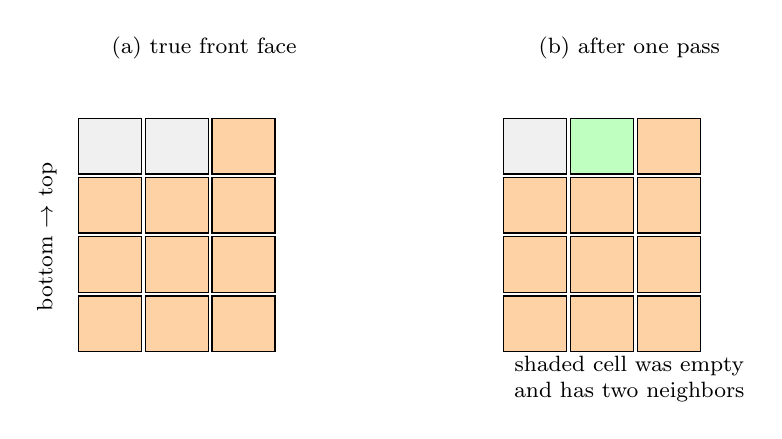
\begin{tikzpicture}[
  font=\footnotesize,
  c/.style={draw, minimum width=8mm, minimum height=7mm, inner sep=0pt, anchor=center},
  on/.style={c, fill=orange!35},
  off/.style={c, fill=black!6},
  add/.style={c, fill=green!25}
]
  \node at (1.2,3.5) {(a) true front face};
  \foreach \r in {0,1,2} {
    \foreach \col in {0,1,2} {
      \node[on] at (\col*0.85, \r*0.75) {};
    }
  }
  \node[off] at (0, 2.25) {};
  \node[off] at (0.85, 2.25) {};
  \node[on] at (1.70, 2.25) {};
  \node[rotate=90, anchor=south] at (-0.55,1.1) {bottom $\rightarrow$ top};

  \begin{scope}[shift={(5.4,0)}]
    \node at (1.2,3.5) {(b) after one pass};
    \foreach \r in {0,1,2} {
      \foreach \col in {0,1,2} {
        \node[on] at (\col*0.85, \r*0.75) {};
      }
    }
    \node[off] at (0, 2.25) {};
    \node[add] at (0.85, 2.25) {};
    \node[on] at (1.70, 2.25) {};
    \node[align=center] at (1.2,-0.7) {shaded cell was empty\\and has two neighbors};
  \end{scope}
\end{tikzpicture}
\caption{The stepped stack of the worked example. The top row truly contains one crate. Gap completion fills the cell beside it and does not fill the corner, because the corner is visited first and has only one orthogonal neighbor at that moment.}
\label{fig:grid}
\end{figure}

The order dependence is visible in the drawing and is easy to overstate. If the pass visited columns from right to left, the middle top cell would still have its lower neighbor and its right neighbor, both original, and would still be filled. The corner would then be visited after the middle cell existed, and would gain a lateral neighbor. A right-to-left pass would fill both empty cells. The implementation visits left to right and therefore fills one. This is a reason to treat the threshold and the visit order as part of the algorithm that was estimated, not as a cosmetic of the pseudocode. A later change to the visit order is a different counter and needs its own row in the table. The present row is the left-to-right, immediate-update, threshold-two counter.

\subsection{A bound on a single false center}
\label{sec:false-center}

One false center can do only a limited amount of damage on a single frame, which is the other half of the argument against the passage union. Suppose the true occupied set is a solid rectangle and the origin is exact. A false center falls either in an occupied cell, in which case the snap ignores the duplicate, or in an empty cell. An empty cell adjacent to the rectangle has at most one orthogonal neighbor inside the rectangle if it shares a side, and it has none if it only touches a corner. The test $n\ge 2$ does not add a side-adjacent cell on the strength of one false center. The false center occupies a cell by itself, and the count grows by $\hat{d}$, once. It does not start a rind.

The passage union removes that limit. Frame $1$ may place a false center on the left of the rectangle and frame $2$ a false center above that false cell, or two frames may place false centers in the same empty side cell and in a second empty cell that becomes its neighbor through the immediate update. Vote threshold one treats each of those as support. The single-frame bound, ``one false center adds at most one cell,'' is false of the union. The estimated bias of $+5.33$ crates for PLC-passage against $+0.83$ for PLC-single is the bound failing in the direction the mechanism predicts. It is also the reason the software specification has no vote accumulator. An accumulator with threshold one is not a harmless extra. It is the counter the estimate rejected.

\subsection{Why the span is the serious baseline}
\label{sec:span-serious}

The mask tally and the area ratio are easy to beat once depth is multiplied in, and a comparison that stopped there would overstate the lattice. The span is the serious baseline because it already knows $(w,h)$ and it already refuses to count raw detections. The three tenths of a crate that separate PLC-single from the span are the entire geometric contribution of the neighbor test, and they should be described at that size.

On a solid rectangle whose corner crates were detected, the span's percentile width and height recover the true number of rows and columns, and the span books $d$ times that product. PLC books the same product if every interior hole was restored and no phantom was added. The two counters differ when the outline is not a solid rectangle, when a false center stretches a percentile, or when an interior miss is common and the span, which does not look inside the rectangle, cannot tell a hole from a filled cell. The stepped top row is the first case. A false center just outside the left column is the second: the second percentile of $x$ moves, $\hat n_c$ in~\eqref{eq:span} can increase by one, and the span multiplies a whole extra column by the number of rows and by $\hat d$. PLC snaps that false center into one cell. If the cell has fewer than two neighbors it stays a single phantom, not a column. The neighbor test is a limit on how much one false center can inflate the count, which is the same limit Section~\ref{sec:false-center} stated from the other direction, and it is the reason a method with a slightly higher exact-match rate can still be the one to deploy when the alternative's errors come in whole columns.

None of this makes the span a straw man. On the loads the generator actually draws, most faces are nearly solid, the span's mean absolute error is $3.31$ against PLC-single's $3.01$, and a deployer who implemented only the span would have captured most of the gain over mask-times-depth. The thesis still specifies the neighbor test, because the extra code is a double loop over a few dozen cells, because the bias drops from $+1.60$ to $+0.83$, and because the failure mode of an extra column is worse than the failure mode of a single phantom cell on a step. The specification would be different if the estimate had gone the other way. It did not.

\begin{figure}[p]
\centering
\begin{tikzpicture}[
  font=\small,
  box/.style={draw, rounded corners=2pt, align=center, inner sep=5pt, minimum width=32mm, minimum height=12mm},
  arr/.style={-{Stealth}, thick}
]
  \node[box, fill=black!6] (det) {Detections\\$m_{\star}-q+f$};
  \node[box, fill=green!15, right=14mm of det] (rule) {Gap rule\\$+r$ restorations\\$+p$ phantoms};
  \node[box, fill=orange!15, right=14mm of rule] (front) {Front count\\$m$};
  \node[box, fill=blue!10, below=16mm of front] (book) {Booked total\\$\hat d \cdot m$};
  \node[box, fill=red!8, left=14mm of book] (depth) {Depth reading\\correct, or $\pm 1$};
  \node[box, fill=black!4, left=14mm of depth] (truth) {Truth\\$N=d\,m_{\star}$};
  \draw[arr] (det) -- (rule);
  \draw[arr] (rule) -- (front);
  \draw[arr] (front) -- (book);
  \draw[arr] (depth) -- (book);
  \draw[arr, dashed] (truth) -- (book);
  \node[align=center, font=\footnotesize] at ($(det.south)+(0,-0.9)$) {misses $q$,\\false cells $f$};
  \node[align=center, font=\footnotesize] at ($(truth.south)+(0,-0.85)$) {signed error\\$\hat N-N$};
\end{tikzpicture}
\caption{How a booked count is assembled, in the letters of~\eqref{eq:front-signed}. The detector contributes misses and false cells. The gap rule puts some misses back and may add phantoms. Depth scales the front count and, when the reading is wrong, adds or removes a whole rank. The dashed arrow is the comparison the estimate computes. It is not an input to the system.}
\label{fig:balance}
\end{figure}
